In multi-tenancy \textit{variability} is a key concept. The term was first introduced in the car industry, where customers could choose certain \textit{variants} of chassis, engine and color~\cite[p. 153]{kabbedijk2011variability}. 
In research on software engineering the concept was defined as ``the ability of a software system or artefact to be efficiently extended, changed, customized or configured for use in a particular context''~\cite{svahnberg2005taxonomy}.
Two keywords from this definition are customization and configuration. 
In a multi-tenant context, configuration is preferred over customization~\cite{sun2008software}, as customization requires the process of reengineering an application, maintaining multiple branches and deploying these branches separately, while configuration can be done at run-time and does not require multiple instances or branches.

\subsection{Why is variability needed}
%reasons for variability [5]
There are several reasons why variability is needed. 
First of all based on country, segment or branch different currencies, legislation and tax rules may apply. This is especially important in financial applications. 
Secondly, different customers can require different functional properties, layout options and/or quality of service (such as privacy and performance).
% MAYBE-TODO: this paragraph could be more elaborate

\subsection{Levels of variability}
%different papers describe different categorizations
Variability can be accomplished on various levels. 
Dependent on the scale of the application, different patterns become relevant. Large applications often consist of \textit{components} offering a specific \textit{service}. Variability can be accomplished by dynamically swapping, activating or deactivating  these components for different tenants in such applications~\cite{mietzner2008defining}. 

In smaller applications and within components, different patterns become relevant. For example, one can customize an application by using dependency injection~\cite{walraven2011middleware} or context oriented programming~\cite{truyen2012context}. We will discus these techniques in more detail in Section~\ref{sec:vrt}.

When looking to realized variability, two types of variability can be distinguished: external and internal variability~\cite{mietzner2009variability}:
\begin{itemize}
\item \textbf{External variability} is the variability that is communicated to the customers. Most of the time, this variability is \textbf{Customer-driven} and is implemented because customers asked for it or because the developers thought the customers would ask for it. The possibility to upload a custom logo, to select data-separation-requirements (such as guaranteed data isolation) or to define custom workflows are examples of external variability.
\item \textbf{Internal variability} exists because of implementation details, is visible only to the developer or provider and is mostly \textbf{Realization-driven}. For example some - external - variant may depend on some internal variation, that guarantees a certain property. When one tenant requires its data to be stored separately, the internal variability consists of the possibility to launch either a single or multiple instances of the database server. It might be more economic to use the same internal variant for all tenants on the same instance to accomplish different external variations, even if this internal variant alone is more expensive.
\end{itemize}
In Section \ref{sec:vrt}, Figure~\ref{fig:ovm} displays this distinction too.  

\subsection{Variability Modeling}
For all stakeholders in a multi-tenant application it is important that a variability model exists~\cite{schroeter2012towards}. For the developer, it is important to document all variation built into the application to keep the application maintainable for both current and new developers. 
For SaaS providers, it is important to have a model of the application to build rules for automatically deploying new instances of the application that support (many) new tenants or migrating and reconfiguring instances. 
Additionally, a model can be used to automatically create configuration wizards~\cite{mietzner2008generation} and bill tenants according to the used variants.
For tenants, it is important that they can use the best tailored variant of the application for their needs and thus it is in their interest too that the SaaS provider has a good overview of its own application and to have a good configuration tool.

To support negotiation about variability in functionality Schroeter et al.~\cite{schroeter2012towards} identified three appropriate models: feature modeling~\cite{benavides2010automated,kang1990feature}, decision modeling~\cite{schmid2004customizable,schmid2011comparison} and orthogonal variability modeling~\cite{lauenroth2005software,metzger2007disambiguating}.

\begin{itemize}
\item \textbf{Feature modeling} or a ``feature based component model" is applied by Walraven et al.~\cite{walraven2011middleware} in their paper on a multi-tenant middleware layer. A variation is
expressed in terms of a feature, a distinctive functionality, service, quality or characteristic of an 
application. Features can have multiple implementations that can then be composed into the 
base application as ideally they are modular pieces of software. By splitting the application in 
these kind of features it is easier to keep functionality together, to make each feature 
customizable and to add implementations in a later stage.

\item \textbf{Decision modeling}, as described by Schmid et al.~\cite{schmid2004customizable}, is used in 
Software Product Line Engineering to manage the variability of an application that is not specifically 
multi-instance or even multi-tenant aware. However the concepts can be similarly applied to 
multi-tenancy. In the decision model, variables are defined that are used throughout the 
application. For each variable it is defined when the variable is relevant (e.g., dependencies), 
what the range of possible values is, what the cardinality is (a set of values is possible), what 
constraints apply and when the variable is to be bound. The problem with decision variables is 
that the configuration points and the application code can quickly become incomprehensible 
when lots of variables exist that might be used thorough different features and components.

\item \textbf{\acf{OVM}} is used by Mietzner et al.~\cite{mietzner2009variability} as their variability model. \ac{OVM} differs from other approaches in that it does provide a separate view on variability. This reduces the size of the model and makes it easier to understand the models as commonalities are left out and only the variability is modeled. This allows for understanding the model without understanding the application's design model. 

\begin{figure}[htr]
    \centering
    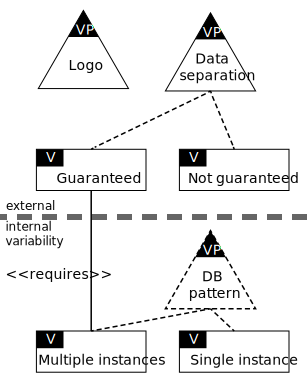
\includegraphics[width=0.48\textwidth]{assets/OVM}
    \caption{Example of a Variability Model in \acs{OVM} notation~\cite{mietzner2009variability}}
    \label{fig:ovm}
\end{figure}

In \ac{OVM}, the \textit{\acp{VP}} are the key items. One variation point has multiple \textit{variants} that are either optional or mandatory. Relations between \acp{VP} exist that define whether some variant is mutually exclusive with some other variant or whether some variant requires an other variant. Relations are drawn as lines between \acp{VP}. External and internal variability are separated by a dashed line to show which variability customers can choose and which is internally bound. An example can be seen in Figure \ref{fig:ovm}.
\end{itemize}

% \subsection{Developing with variability in mind}
% Efficient customization of multi-tenant Software-as-a-Service applications with service lines
% by Stefan Walravena, Dimitri Van Landuyta, Eddy Truyena, Koen Handekynb, Wouter Joosena

\subsection{\aclp{VRT}}
\label{sec:vrt}
Jansen et al.~\cite{jansen2010customization} note that while lot of research has been done on variability modeling, there is lack of research on techniques needed to implement variability. They divide \acp{VRT} in two categories, with further subdivisions:
\begin{itemize}
\item \textit{\ac{MVC} Customization}
\begin{itemize}
\item \textbf{Model changes} allow tenants to fit the application to their domain. Model changes include changing entity attributes, adding entities and entity-relationships. Some changes require a more abstract application and therefore need to be thought upon earlier in the design process than more simple changes which could easily be added later on.
\item \textbf{View Changes} is one of the simpler types of customization, because in the \ac{MVC}-pattern, views do not interact with other components, but instead receive the data to be displayed.
\item \textbf{Controller Changes} allow the most freedom, ranging from restricting data to one tenant only, till fully customized workflows.
\end{itemize}
\item \textit{System Customization} \\ Within large systems, built of components delivering services, variations of a different magnitude can be created, on system level.
\begin{itemize}
\item \textbf{System Connector Changes} occur when connections to remote services are made variable. Examples include having multiple connectors for printing photos or multiple physical mail delivery providers.
\item \textbf{System Component Changes} require that multiple components deliver the same service. Based on the configuration, one of the components for a service is selected. For example tenants might select different authentication components for either SAML\footnote{Security Assertion Markup Language - \url{http://en.wikipedia.org/wiki/Security_Assertion_Markup_Language}}, OAuth\footnote{Open Authorization - \url{http://en.wikipedia.org/wiki/OAuth}} or password-based login.
\end{itemize}
\end{itemize}

Kabbedijk and Jansen~\cite{kabbedijk2011variability} describe three \acp{VRT} they observed in case studies. These \acp{VRT}  fit into the categories above.
\begin{itemize} 
\item \textbf{Customizable Data Views}: a pattern to store tenant specific representation settings, e.g. how tenants want to filter or sort their data. 
Although this technique requires some table storing data and needs a small controller, it can be seen as mainly a View Change.
\item \textbf{Module Dependent Menu}: modules can add items to the menu. Depending on which modules are associated with a tenant, the menu is thus customized. This is another View Change pattern. 
\item \textbf{Pre/Post Update Hooks}: execute pieces of code before or after certain events happen in the application. This is a Controller Change. 
This allows for tenants to enable or disable modules that check data or automate certain tasks.
\end{itemize}

Two ways to implement Controller Changes or System Component Changes are \acl{DI} and \acl{COP}.

\textbf{\acf{DI}} is a variation technique, where one of the (possibly many) classes that implement the same interface are injected by a provider. Tools such as Spring Framework~\cite{walls2005spring} and Google Guice~\cite{vanbrabant2008google} provide a framework for \ac{DI}. The main use case of \ac{DI} is mocking components while testing an application, however it proves useful in multi-tenant applications as well:
Walraven et al.~\cite{walraven2011middleware} created a multi-tenancy middleware layer that uses Guice, which is compatible with \ac{GAE}. An issue with Guice, that did not allow per-request switching of implementations, was quickly solved by adding a small abstraction layer, making Guice usable in a multi-tenant environment\footnote{
Additionally, their case study shows that \ac{GAE} leverages the effort of separating tenant data a lot by providing the so-called Namespaces API. By linking each tenant to an unique namespace all data in that namespace is only accessible by a that specific tenant.}.

One of the conclusions of Walraven et al.~\cite{walraven2011middleware} is that \ac{AOSD} looks promising as an alternative to \ac{DI} for more complex customizations, such as when features have to be combined.
They go further on this lead in Truyen et al.~\cite{truyen2012context} and introduce \textbf{\ac{COP}}, a form of \ac{AOSD} to implement what can be seen as controller changes. 
In \ac{COP}, layers are added to the code that override certain behavior when this layer is activated for a specific tenant. 
In \ac{DI}, for each variation point only one variation can be injected at a time, so no two `modules' providing the same functionality can interact or extend each other, while in \ac{COP} those implementations can work together, because the overriding methods can still call the original method allowing them to modify the output or implement a filter. 
Multiple layers can be active at once, doing their work in a predefined order.
% MAYBE-TODO: this paragraph could be more elaborate

\subsection{Research Agenda for Variability}\label{sec:var_agenda}
While there has been done a lot of research, much remains to be covered:
\begin{itemize}

\item \textbf{Automation}.
For variability to become manageable, tools must exist for \ac{SaaS} providers to manage the configuration of tenants and to deploy new tenants. Mietzner et al. try to make variability easier to manage by creating so called \textit{customization processes}~\cite{mietzner2008generation} to guide the customer through the customization, and \textit{solutions}~\cite{mietzner2008defining}, that define which variants should be bound. It could be investigated how deployment scripts could be derived from these solutions, to automatically deploy tenants.

\item \textbf{Cost Models}.
While it is researched how the costs of multi-tenant aware applications compare to non-multi-tenant aware applications~\cite{mietzner2009variability}, no research is done to relate a cost model to a variability model. Future research could be done to determine the cost of creating, maintaining and managing variants. The providers can then decide whether or not it makes more sense, economically, to keep a variant or to remove it.

\item \textbf{Identify more \aclp{VRT}}. 
Kabbedijk and Jansen~\cite{kabbedijk2011variability} have determined some \acp{VRT}, but note that more \acp{VRT} could be identified and should be tested on effectiveness, maintainability, scalability and performance.

\item \textbf{Maintaining Context in \ac{COP}}. 
Truyen et al.~\cite{truyen2012context} found that \ac{COP} was useful as a \ac{VRT} but ContextJ lacked support for asynchronous request because context is not shared to new threads. Research could be done to see if it is possible to bridge this gap to make \ac{COP} more usable as more and more applications are using asynchronous functionality.

\item \textbf{Maintaining State Consistency while doing Updates}.
Another open issue is maintaining global state consistency when doing (partial) updates of components that potentially service a lot of tenants~\cite{truyen2012context,dumitracs2009upgrades}. The tenants that do not use any of the updated functionality should not experience any interruptions. This is especially difficult if multiple versions of components must coexist, since each component may depend on other components. When \acp{SLA} are sold this consistency and uninterrupted service should be provable.

\end{itemize}
% schroeter2012towards